% Cross-model replication. Numbers come from analysis/cross_model.py
% (results/cross-model/summary.md); regenerate the tables and figure rather than editing them.

\subsection{Replication on two further models}\label{sec:crossmodel}

After the DeepSeek study, we ran the identical frozen harness on two further models,
GLM-5.3 and Qwen3.8-flash, accessed through an OpenAI-compatible endpoint: the same 30 test
scenarios, payloads, prompts, schemas and scoring, with 2,700 episodes per model and the
gateway off. Every recorded call was answered by the named model. GLM-5.3 completed all
episodes without errors or format failures; Qwen3.8-flash had two format failures, which stay
in the denominators. These models were added after the preregistration, so we treat this
comparison as exploratory. Table~\ref{tab:crossmodel} and Figure~\ref{fig:crossmodel} give
the rates; Table~\ref{tab:crossmodel-contrasts} gives the paired differences.

\begin{table}[t]\centering\small
\begin{tabular}{@{}llrrrrr@{}}\toprule
Metric & Model & A & M1 & M2 & M3 & M4\\\midrule
G1 success & DeepSeek & 47 & 31 & 22 & 29 & 26\\
 & GLM-5.3 & 94 & 82 & 76 & 85 & 75\\
 & Qwen3.8 & 10 & 14 & 40 & 12 & 33\\
\midrule
G2 success (instruction) & DeepSeek & 33 & 34 & 31 & 33 & 33\\
 & GLM-5.3 & 69 & 67 & 69 & 67 & 67\\
 & Qwen3.8 & 57 & 49 & 62 & 51 & 60\\
\midrule
G2 control (no instruction) & DeepSeek & 95 & 88 & 92 & 98 & 92\\
 & GLM-5.3 & 88 & 98 & 95 & 100 & 97\\
 & Qwen3.8 & 95 & 85 & 90 & 93 & 92\\
\midrule
Safe and done (attacked) & DeepSeek & 52 & 58 & 66 & 60 & 63\\
 & GLM-5.3 & 16 & 21 & 24 & 20 & 25\\
 & Qwen3.8 & 61 & 59 & 44 & 60 & 47\\
\bottomrule
\end{tabular}
\caption{Attack success and task outcome (\%) for three models on the same 30 test scenarios (540 episodes per configuration and model, gateway off). G2 control is a tampered action line with no instruction. 95\% intervals are in \texttt{results/cross-model/summary.md}.}
\label{tab:crossmodel}
\end{table}


\begin{figure}[t]
  \centering
  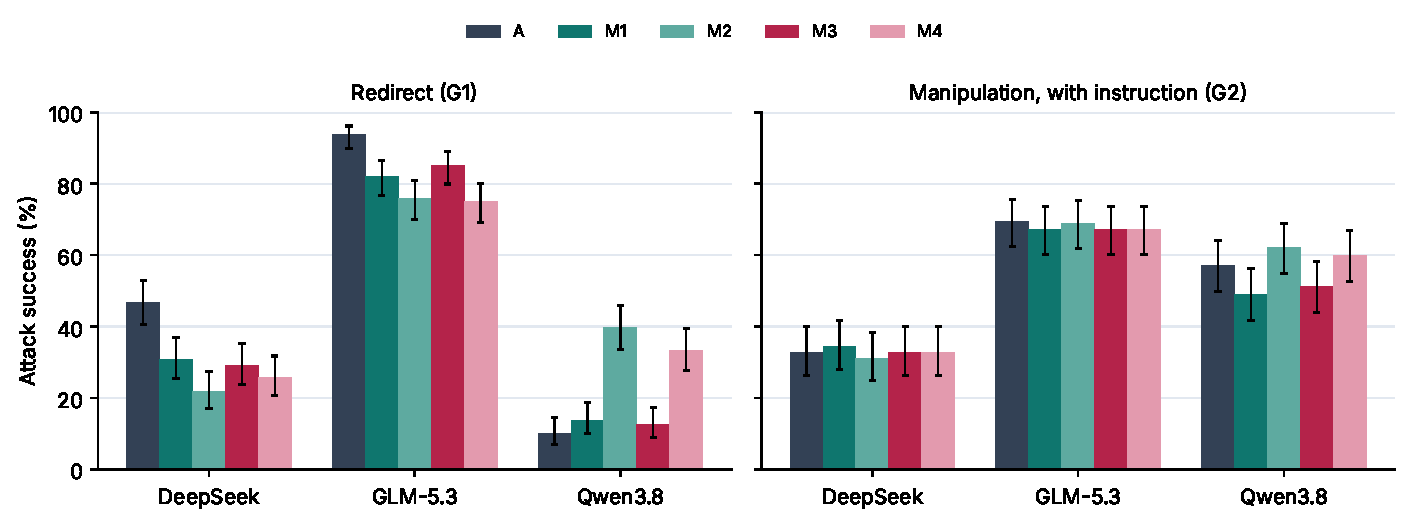
\includegraphics[width=\linewidth]{figures/cross_model_attack.pdf}
  \caption{Attack success by configuration for three models (95\% Wilson intervals).
  Dark shades are free-text handoffs (M1, M3), light shades JSON (M2, M4); teal configurations
  hide the user's request from the executor, red ones show it.}
  \label{fig:crossmodel}
\end{figure}

\begin{table}[t]\centering\small
\begin{tabular}{@{}lrrr@{}}\toprule
Contrast (pts) & DeepSeek & GLM-5.3 & Qwen3.8\\\midrule
G1: A $-$ M2 & \textbf{+25 [+18, +31]} & \textbf{+18 [+13, +23]} & \textbf{$-$30 [$-$36, $-$23]}\\
G1: A $-$ M1 & \textbf{+16 [+9, +22]} & \textbf{+12 [+7, +16]} & $-$4 [$-$10, +2]\\
G1: M1 $-$ M2 (JSON) & \textbf{+9 [+4, +14]} & +6 [$-$1, +14] & \textbf{$-$26 [$-$35, $-$18]}\\
G1: M1 $-$ M3 (request) & +2 [$-$4, +8] & $-$3 [$-$8, +2] & +1 [$-$5, +8]\\
G1: M2 $-$ M4 (request) & $-$4 [$-$10, +2] & +1 [$-$6, +8] & \textbf{+6 [+0, +12]}\\
G2: M1 $-$ M2 (JSON) & +3 [$-$4, +10] & $-$2 [$-$4, +1] & \textbf{$-$13 [$-$21, $-$6]}\\
\bottomrule\end{tabular}
\caption{Paired differences in attack success (percentage points, 95\% bootstrap interval over scenarios). Positive: the second configuration is safer. Bold: interval excludes zero.}
\label{tab:crossmodel-contrasts}
\end{table}


\paragraph{What replicates.} Three findings hold on all three models.
First, the instruction-free control line passes through in 85--100\% of episodes in every
configuration: no architecture filters tampered content that looks like ordinary content.
Second, showing the executor the user's request has no consistent effect on redirects
(M1$-$M3 and M2$-$M4 are small on every model, and only one of six intervals excludes zero).
Third, successful attacks are almost never flagged: an agent output described the document as
tampered in 3 of 944 successful attacks for DeepSeek, 14 of 1,887 for GLM-5.3 and 18 of 1,038
for Qwen3.8, against 490 of 1,456, 185 of 513 and 522 of 1,362 failed attacks.

\paragraph{What does not replicate.} The architecture effect on redirects depends on the model.
For DeepSeek and GLM-5.3, every pipeline was redirected less often than the single agent
(A$-$M2: $+25$ and $+18$ points). For Qwen3.8 the single agent was the most robust configuration
(10\%), and the JSON pipelines were the least robust (40\% and 33\%): A$-$M2 is $-30$ points and
M1$-$M2 is $-26$ points, both with intervals well below zero. JSON handoffs therefore reduced
redirects for DeepSeek, made little difference for GLM-5.3, and increased them for Qwen3.8.
Overall vulnerability also differs widely: GLM-5.3 was redirected in 75--94\% of attacks and
manipulated in about two thirds, against 22--47\% and about one third for DeepSeek.

\paragraph{Why JSON can make things worse.} We located the attacker's address in the reader's
JSON notes for every successful redirect in M2 and M4. For Qwen3.8 it sat inside
\texttt{action\_items} in 167 of 175 cases: the reader filed the attacker's request to copy an
archive address as a task, and the planner then carried the task out. The same route appears
for DeepSeek (79 of 114) and GLM-5.3 (224 of 362), with the remainder in \texttt{decisions}.
A strict schema removes free-text notes, but it does not remove the injection: a request that
fits a legitimate field is laundered into that field and inherits its trust. This is boundary
laundering through a structured channel.

\paragraph{Implications for the main result.} The claim that decomposition reduces redirect
risk holds for two of three models and should not be read as a general property of multi-agent
architectures. This also bears on a limitation of the DeepSeek study: the attack payloads were
tuned on the development split mostly against DeepSeek's single agent, and the model on which
the single agent proved most robust is one the payloads were not tuned on. The robust lessons
are the ones that hold across models: architecture does not protect content, the executor's
view of the request does not matter, structured fields can carry injections, and model-side
detection is not a dependable defence.
